\documentclass{standalone}
\usepackage{tikz}
\usetikzlibrary{shapes.geometric, arrows}

\tikzstyle{arrow} = [thick,->,>=stealth]

\begin{document}

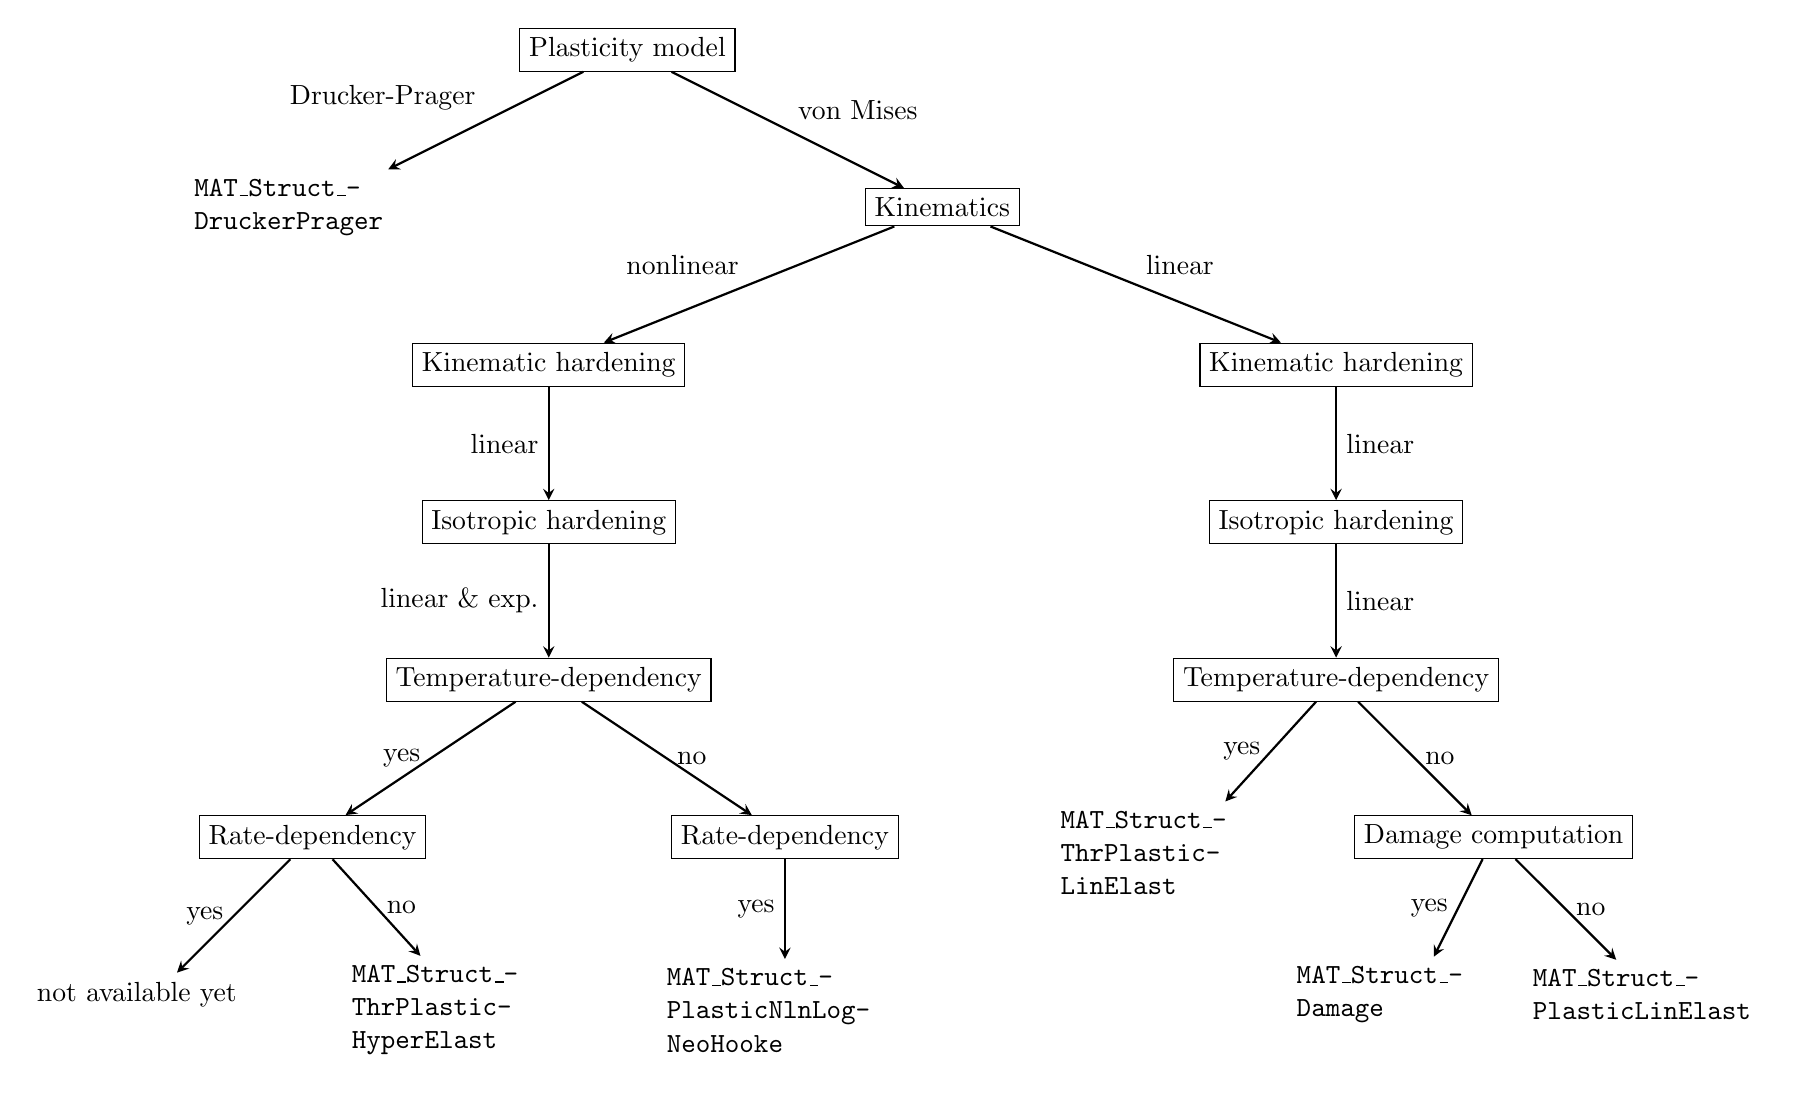
\begin{tikzpicture}[node distance=2cm]

\node[rectangle, draw] (start_0) at (-4, 2) {Plasticity model};

\node[rectangle, draw] (start) at (0,0) {Kinematics};

\draw [arrow] (start_0) -- node[anchor=south west] {von Mises} (start);

\node[text width=3cm] (druckerprager) at (-8,0) {\texttt{MAT\_Struct\_\-Drucker\-Prager}};

\draw [arrow] (start_0) -- node[anchor=south east] {Drucker-Prager} (druckerprager);

% left side

\node[rectangle, draw] (kinhard_l) at (-5,-2) {Kinematic hardening};
\node[rectangle, draw] (isohard_l) at (-5,-4) {Isotropic hardening};
\node[rectangle, draw] (thermo_l) at (-5,-6) {Temperature-dependency};
\node[rectangle, draw] (rate_ll) at (-8,-8) {Rate-dependency};
\node[rectangle, draw] (rate_lr) at (-2,-8) {Rate-dependency};

\node[text width=3cm] (notavail) at (-10,-10) {not available yet};
\node[text width=3cm] (threlasthyper) at (-6,-10.2) {\texttt{MAT\_Struct\_\-ThrPlastic\-HyperElast}};
\node[text width=3cm] (logneohooke) at (-2,-10.2) {\texttt{MAT\_Struct\_\-Plastic\-NlnLog\-NeoHooke}};

\draw [arrow] (start) -- node[anchor=south east] {nonlinear} (kinhard_l);
\draw [arrow] (kinhard_l) -- node[anchor=east] {linear} (isohard_l);
\draw [arrow] (isohard_l) -- node[anchor=east] {linear \& exp.} (thermo_l);
\draw [arrow] (thermo_l) -- node[anchor=east] {yes} (rate_ll);
\draw [arrow] (thermo_l) -- node[anchor=west] {no} (rate_lr);
\draw [arrow] (rate_ll) -- node[anchor=east] {yes} (notavail);
\draw [arrow] (rate_ll) -- node[anchor=west] {no} (threlasthyper);
\draw [arrow] (rate_lr) -- node[anchor=east] {yes} (logneohooke);

% right side

\node[rectangle, draw] (kinhard_r) at (5,-2) {Kinematic hardening};
\node[rectangle, draw] (isohard_r) at (5,-4) {Isotropic hardening};
\node[rectangle, draw] (thermo_r) at (5,-6) {Temperature-dependency};
\node[rectangle, draw] (damage_r) at (7,-8) {Damage computation};

\node[text width=3cm] (thrlinelast) at (3,-8. 2) {\texttt{MAT\_Struct\_\-ThrPlastic\-LinElast}};

\node[text width=3cm] (damage) at (6,-10) {\texttt{MAT\_Struct\_\-Damage}};
\node[text width=3cm] (linelast) at (9,-10) {\texttt{MAT\_Struct\_\-Plastic\-LinElast}};

\draw [arrow] (start) -- node[anchor=south west] {linear} (kinhard_r);
\draw [arrow] (kinhard_r) -- node[anchor=west] {linear} (isohard_r);
\draw [arrow] (isohard_r) -- node[anchor=west] {linear} (thermo_r);
\draw [arrow] (thermo_r) -- node[anchor=west] {no} (damage_r);
\draw [arrow] (thermo_r) -- node[anchor=east] {yes} (thrlinelast);
\draw [arrow] (damage_r) -- node[anchor=east] {yes} (damage);
\draw [arrow] (damage_r) -- node[anchor=west] {no} (linelast);

\end{tikzpicture}
\end{document}
